\chapter{Vorbereitung}

\section{Theoretische Grundlagen zum AFM}
       
Beim Rasterkraftmikroskop sind die Kräfte ,die die Probe, auf atomarer Ebene auf einen Messkopf wirken, entscheidend.

 \subsection{Kräfte zwischen Atomen}
        \subsubsection{Van-der-Waals Kräfte}

Die Ladungsverteilung in Atomen ist nicht konstant, sondern unterliegt ständiger 
Fluktuation. Der Schwerpunkt der negativen Ladungen kann hierbei vom dem der
positiven Ladungen abweichen. Ist dies der Fall, so entsteht ein Dipol. 
Befindet sich nun ein zweites Teilchen in der Nähe dieses Atoms, so wird auch
in diesem ein Dipol induziert. Zeigt die positive Seite des ersten Atoms zu Atom 2,
so werden die Elektronen des zweiten Atoms angezogen. Ist es die negative Seite, so
werden die Elektronen abgestoßen. 
\vspace{3pt}\\
Als Folge dessen synchronisieren sich die Ladungsänderungen der beiden Atome. Eine
schwache positive Anziehung ist die Folge. Diese ist proportional zu $\displaystyle
\frac{-1}{r^6}$.

        \subsubsection{Pauli-Abstoßung}

Nähern sich die Atome weiter an, so kommt es zu einem Überlappen der 
Elektronenorbitale. Das Pauli-Verbot verhindert hierbei, dass zwei Elektronen den
gleichen Zustand besetzen. Einige Elektronen werden folglich in einen energetisch
höheren Zustand gezwungen. \\
So führt eine Orbitalüberlagerung zu einer repulsiven Wechselwirkung. Die Kraft
ist proportional zu $\displaystyle \frac{1}{r^{12}}$.

        \subsubsection{Lennard-Jones Potential}

Bei sehr kleinen Abständen dominiert die Pauli-Abstoßung, bei größeren die 
van-der-Waals Kräfte. Die Summe aus beiden Potentialen wird Lennard-Jones 
Potential gennant. 
\[
   \phi (r) \propto \frac{A}{r^6} - \frac{B}{r^{12}}    
\]

Dabei bezeichnet $\phi$ das Potential und somit die Bindungsenergie, r den Abstand.
A, B sind Konstanten die stoffspezifisch sind.

\begin{figure}[h!]
    \centering
    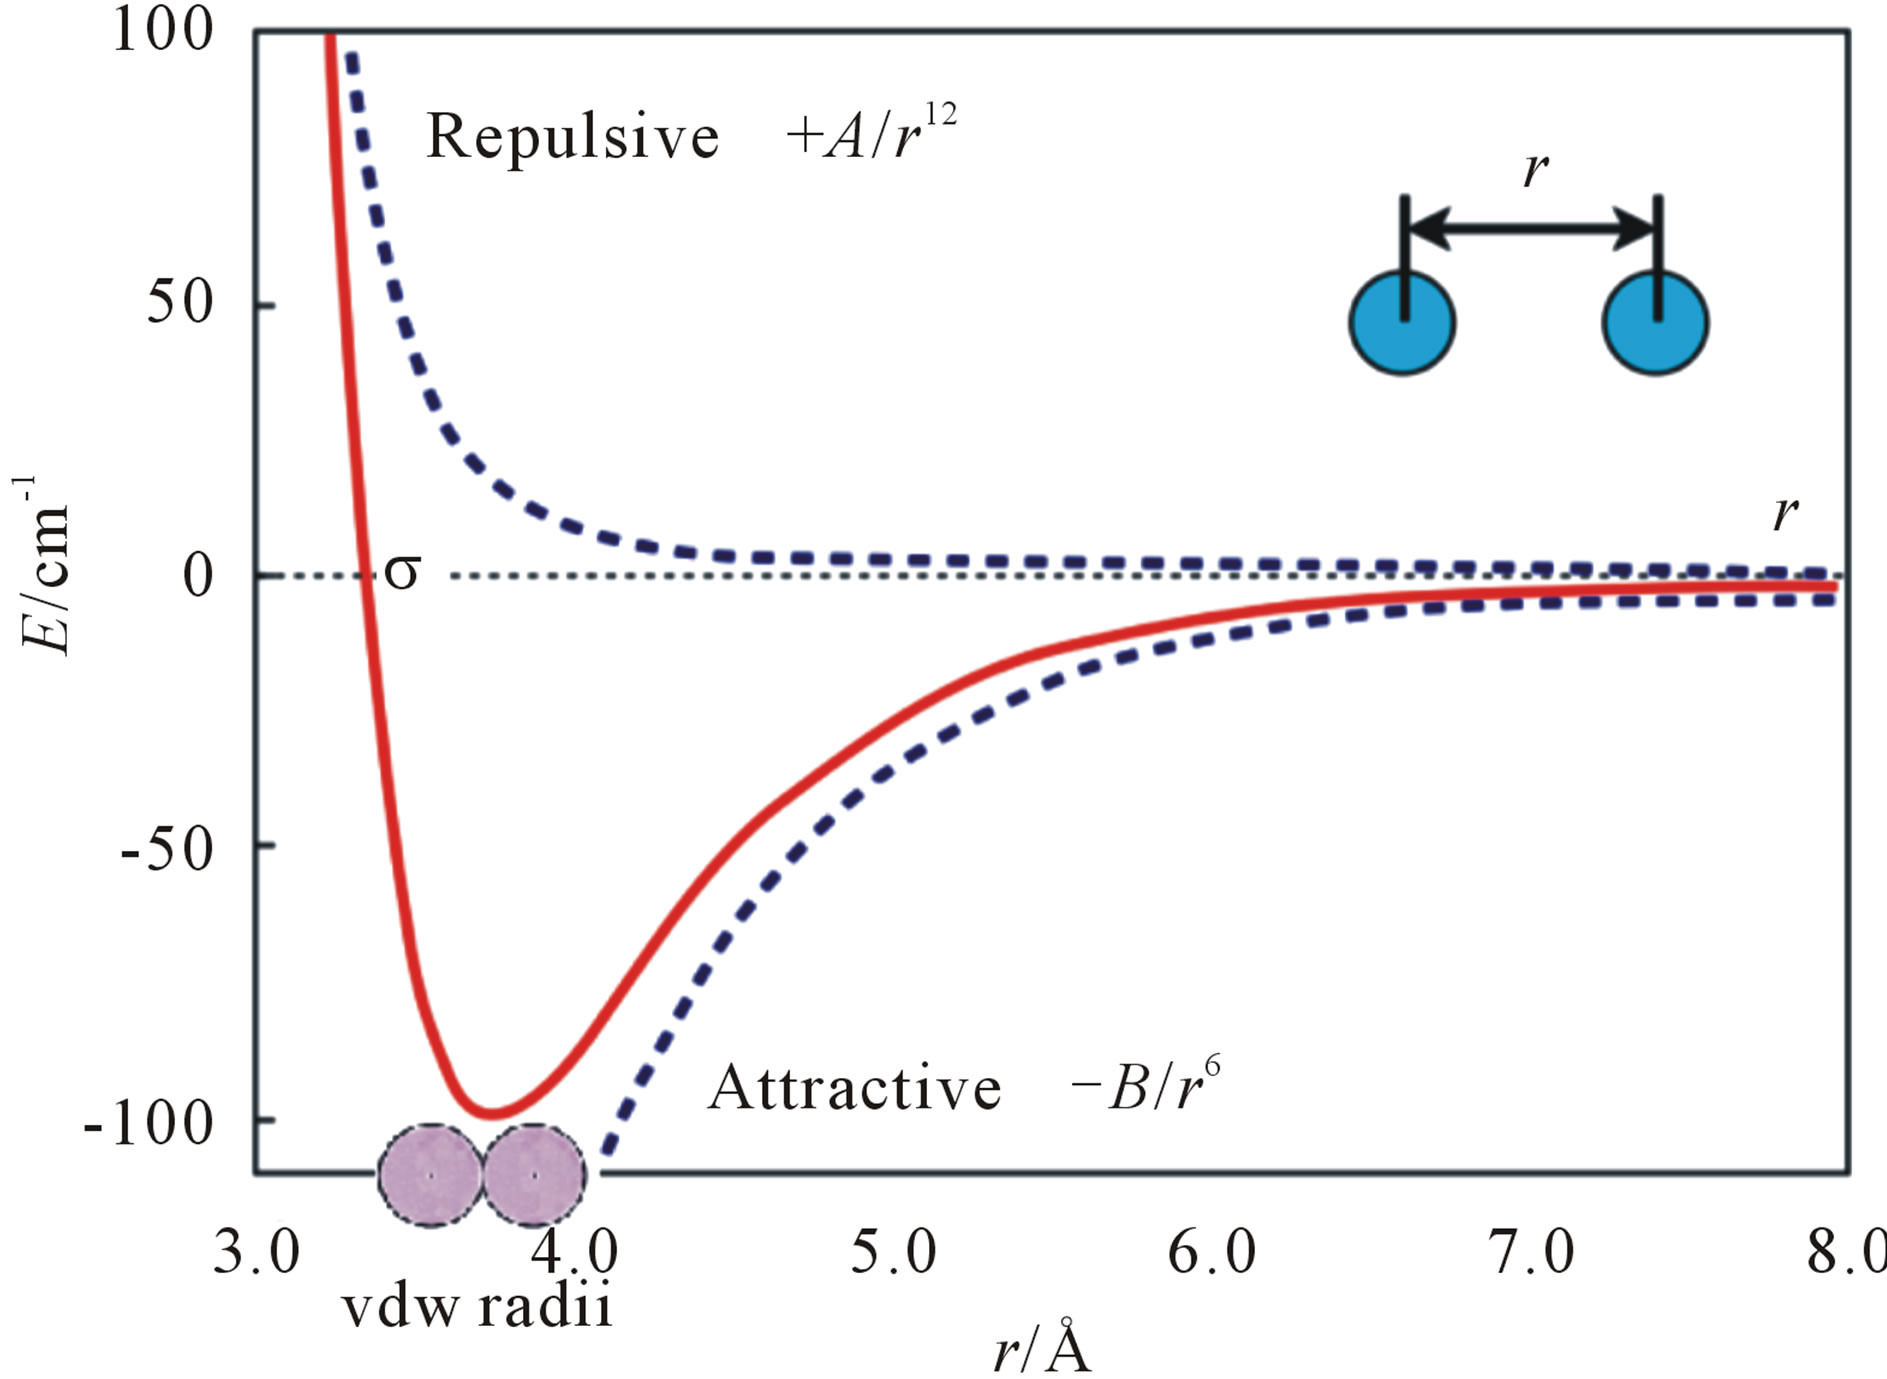
\includegraphics[width=0.6\textwidth]{Abb/ljp.jpg}
    \caption{Das Lennard-Jones Potential als Summe der vdW-Wechselwirkung und
             der Pauli-Abstoßung [https://file.scirp.org/Html/2-8301839/5ea73474-0e91-41d4-a386-71cdc9f14e20.jpg]}
    \label{ljp}
\end{figure}

Neben diesen Kräften können im Allgemeinen auch noch chemische Bindungskräfte, Kontaktkräfte, magnetische und elektrische Wechselwirkungen eine Rolle besitzen.
Bei unserem Aufbau haben sie jedoch nur geringe Bedeutung.



\subsection{Der Cantilever}
\label{herleitung}

 
Der Cantilever ist ein schwingungsfähiger Balken, der eine pyramidale Spitze mit einer Dicke von nur wenigen Nanometern besitzt.
Er wird meist aus $Si_3N_4$ hergestellt und an dessen Ende wird, durch Ätzung, eine abstehende sehr sehr dünne Spitze geformt.
Seine Resonanzfrequenz befindet sich etwa im kHz bis MHz Bereich.
Mit ihm lassen sich nun die bereits besprochenen Abstoßungs- bzw. Anziehungskräfte messen.
Der Cantilever, verhält sich durch seine periodische Bewegung in guter Näherung wie ein getriebener, gedämpfter harmonischer Oszillator. 
Die Formel dazu sieht folgendermaßen aus:
\[
    m \ddot{x} + \frac{m \omega_0}{Q} \dot{x} + kx = F_0 \cos(\omega t)
\]
Wir verwenden hier m als die punktförmig genäherte Masse des Cantilevers, $\omega_0$ ist dessen Eigenfrequenz mit seiner Güte $Q$ und $k$ beschreibt eine Federkonstante die für die rücktreibende Kraft, also die Oszillation, verantwortlich ist.
Auf der rechten Seite der Gleichung beschreibt $F_0$ die treibende Kraft, die die Probe und die Vorrichtung auf den Cantilever wirken.
Wir benutzen den Ansatz:
\[
    x(t)=A \cdot e^{iwt}
\]
und bekommen schließlich durch Einsetzen folgende Gleichung.
\[
   \left(-\omega^2+\omega_0^2-i\frac{\omega_0}{Q} \cdot \omega \right) \cdot A 
   = \frac{F_0}{m}
\]
Löst man diese Gleichung anschließend nach der Amplitude A auf, erhält man 
folgendes Ergebnis:
\[
    A = \frac{F_0}{m \sqrt{ ( \omega_0^2 - \omega^2 )^2 + \left( \frac{\omega 
        \omega_0}{Q} \right)^2}}
\]

Die Auswirkungen auf seine Resonanzkurve bei attraktiver und repulsiver Wechselwirkung lassen sich der Abbildung \ref{vorb_sweep} entnehmen.

\begin{figure}[h!]
    \centering
    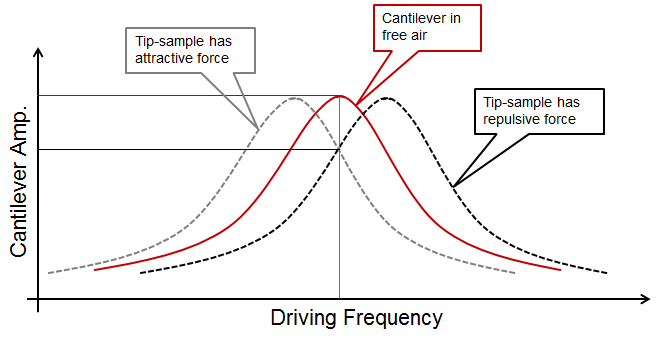
\includegraphics[width=0.6\textwidth]{Abb/freqsweep.png}
    \caption{Resonanzkurve des Cantilevers [https://vetsuisse.com/vet-iml/lernmodule/htmls/slide.html?radiosurfvet|radgeneral|sonography|sonobasics|2]}
    \label{vorb_sweep}
\end{figure}

[https://vetsuisse.com/vet-iml/lernmodule/htmls/slide.html?radiosurfvet|radgeneral|sonography|sonobasics|2]


\section{Betriebsmodi}


Es gibt zwei Methoden um die Kräfte der Probe auf den Cantilever wirken zu lassen.
Es gibt den statischen Modus und den dynamischen Modus. 
Beim statischen Modus wird der Cantilever nicht in Schwingung versetzt und in Ruhe gehalten.
Der dynamische Modus arbeitet hingegen mit einem schwingenden Cantilever.
Der statische Modus ist leichter umzusetzen und war desshalb der Beginn der Rasterkraftmikroskopie, heutzutage verwendet man eher die dynamischen Modi, welche keinen physischen Kontakt mit der Probe benötigen.



\subsection{Statischer Modus:}

Bei dem statischen Betriebsmodus bringt man die Messspitze des Cantilevers in direkten Kontakt mir der Probe.
Der Cantilever verbiegt sich nun entsprechend der attraktiv und repulsiv wirkenden Kräfte.
Dabei regelt der Rastermechnismus die Höhe zu permanentem Kontakt mit der Probe nach.
Man kann allerdings auch die Höhe des Cantilevers über der Probe konstant halten und die Wechselwirkung mit der Probe aufzeichnen.
Der statische Modus hat jedoch Nachteile.
Der Cantilever und die Probe werden dabei beansprucht, oder sogar zerstört.
Auch das Nachregeln der Höhe über die Rastereinheit, kann bei großen Bergen und Tälern die Spitze direkt in die Probe fahren.
Lässt man den Cantilever auf konstanter Höhe, können die Wechselwirkungen zur Probe zu gering sein, um sie messen zu können.

Weil sich bei diesem Modus die Bauteile und die Probe sehr stark abnutzen können, entwickelte man eine Alternative, den dynamischen Modus.

\subsection{Dynamischer Modus:}

       \paragraph{Amplitudenmoduliertes Rasterkraftmikroskop}

Hier versetzt man den Cantilever, nach dem Prinzip des harmonischen Oszillators, in eine Schwingung nahe seiner Eigenfrequenz, sodass abstoßende Kräfte die Resonanzfrequenz erhöhen und anziehende Kräfte die Resonanzfrequenz verringern. 
Würde man den Cantilever bei seiner Eigenfrequenz anregen, würde sowohl attraktive als auch repulsive Kraftwechselwirkung zu einer Absenkug von Amplitude führen, somit wäre eine Zuordnung über attraktive oder repulsive Krafteinwirkung nicht eindeutig. Dies wird in der Graphik \ref{vorb_sweep} veranschaulicht.
Mit der Anregung nahe der Eigenfrequenz, sorgt diese Frequenzänderung nun auch für eine Amplitudenänderung.
Der Cantilever wird über seine z-Koordinate wieder auf seine ursprüngliche Amplitude gebracht, die Amplitudenänderung gibt aber die Kräfte, welche die Probe auf den Cantilever wirkt, eindeutig wieder.

 In unserem Versuch wird die Methode der Amplitudenänderung verwendet. 
Die anziehenden und abstoßenden Kräfte deformieren den Cantilever so stark, dass die Amplitude um bis zu 30\% verringert wird.
(http://www.physik.uni-regensburg.de/studium/praktika/f/fpAFM2010.pdf, 05.11.2019)

       \paragraph{Frequenzmoduliertes Rasterkraftmikroskop}
       
Versetzt man den Cantilever in die Nähe seiner Eigenresonanz, kann man beobachten, dass er neben einer Frequenzänderung auch eine Phasenverschiebung seiner harmonischen Schwingung erfährt.
Bei dem frequenzmodulierten Modus wird nun die Frequenzänderung vermieden, also konstant nahe seiner Eigenfrequenz gehalten.
Die Phasenverschiebung beinhaltet alle notwenigen Informationen für die Nachregelung in z-Richtung und die Auswertung der Probenbeschaffenheit.
Diese Methode machte die Auflösung der Rasterkraftmikroskopie noch um einiges besser, jedoch nicht effizienter.
Ohne Kontakt mit der Probe, kann man mit diesen Modi also auf atomarer Ebene die Beschaffenheit, auch von allen nicht ferromagnetischen Stoffen, messen.
       
 \section{Aufbau des Rasterkraftmikroskops}
\begin{figure}[h!]
    \centering
    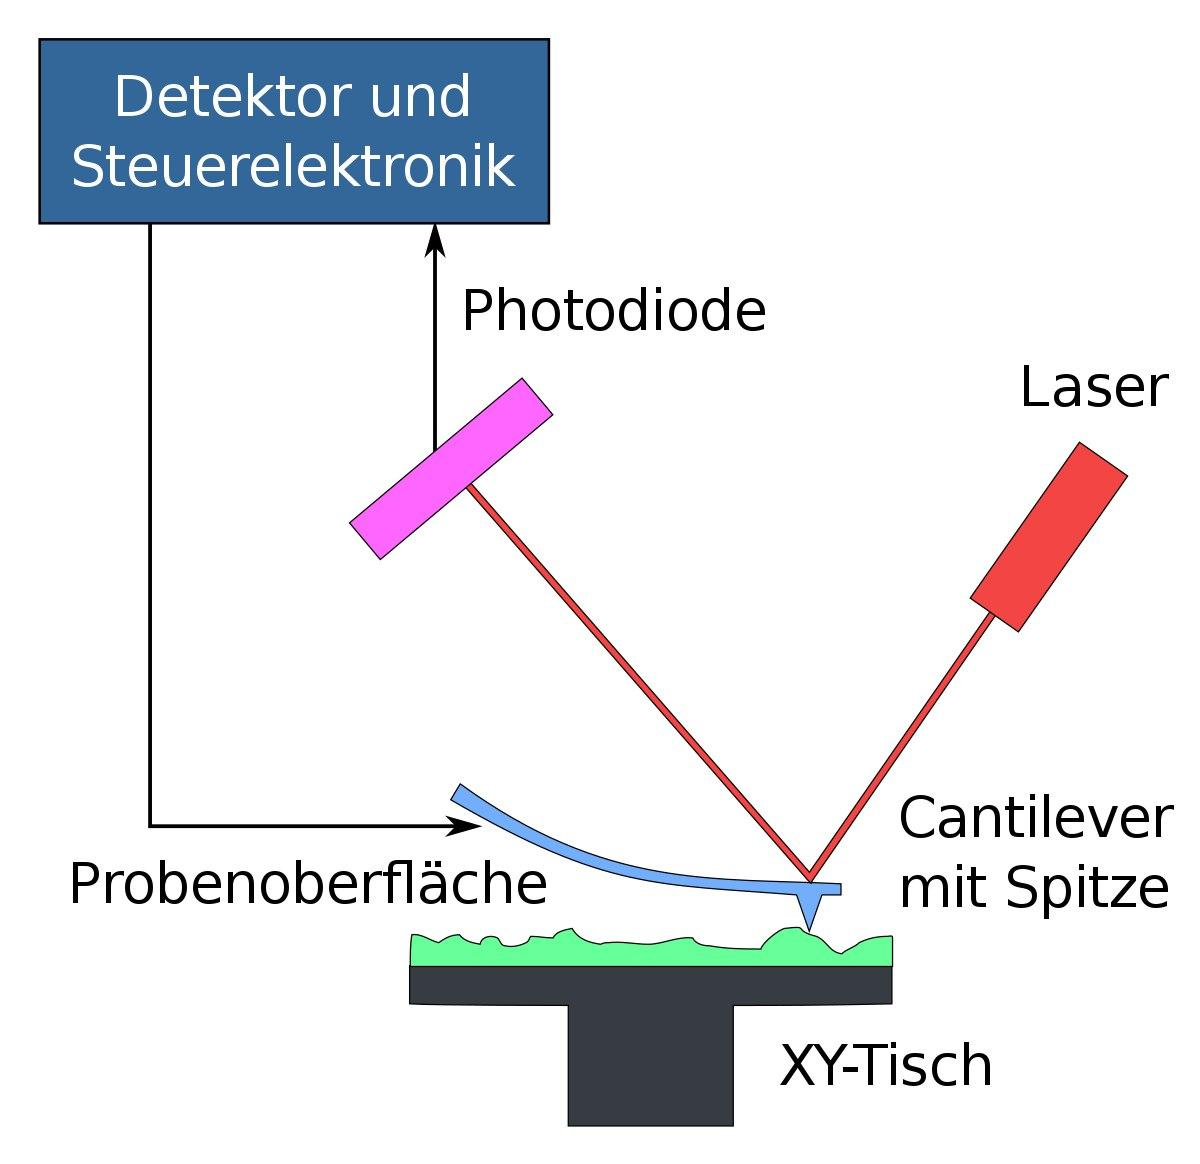
\includegraphics[width=0.6\textwidth]{Abb/afm.jpg}
    \caption{Aufbau eines AFM [https://de.wikipedia.org/wiki/Rasterkraftmikroskop]}
    \label{afm}
\end{figure}

Das verwendete Mikroskop besteht aus einem Cantilever mit Messspitze, einem Positioniersystem für die z-Richtung, einem Positioniersystem für x- bzw. y-Richtung und einer Detektionseinheit, welche die Amplitudenänderung des Cantilevers misst.  
Die Spitze des Cantilevers wird über verschiedene Bauelemente sehr nahe an die Probe gebracht um deren Wechselwirkung zu spüren.
Gleichzeitig versetzt man den Cantilever nahe seiner Resonanzfrequenz und beobachtet über die Detektionseinheit, wie stark diese Schwingung durch die Probe eingeschränkt wird.


\subsection{Rastermechanismus}

Am Anfang fährt man die Probe mittels eines Schrittmotors mechanisch bis auf wenige Mikrometer auf die Probe in z-Richtung heran.
Anschließend nutzt man den piezoelektrischen Effekt um eine feinere Ansteuerung zu ermöglichen.
Zumeist verwendet man piezoelektrische Röhrchen aus Blei-Zirkonat-Titanat, denn dieses Material kann sich mithilfe einer angelegten Spannung stark dehnen und zusammenziehen. 
Die Spannung am piezoelektrischen Röhrchen wird über die Rückkopplung mit dem Cantilever gesteuert. 
Um den piezoelektrischen Effekt und sein Inverses korrekt verstehen zu können, muss man auf atomare Ebene dieser Moleküle die Ladungsverschieben betrachten.
Bei diesem Effekt geht es konkret darum, dass man bei äußerlicher Krafteinwirkung auf bestimmte Kristallstrukturen, eine Spannung innerhalb dieser Kristalle messen kann.
Die Ursache hierfür ist, dass durch die mechanische Krafteinwirkung die Ladungsverteilung innerhalb von Kristall-Elementarzellen verschoben wird.
Dadurch ergibt sich ein Dipol, welcher eine elektrische Kraft resultiert.
Für besseres Verständnis ist dies in Abbildung \ref{piezo} zu sehen.

\begin{figure}[h!]
    \centering
    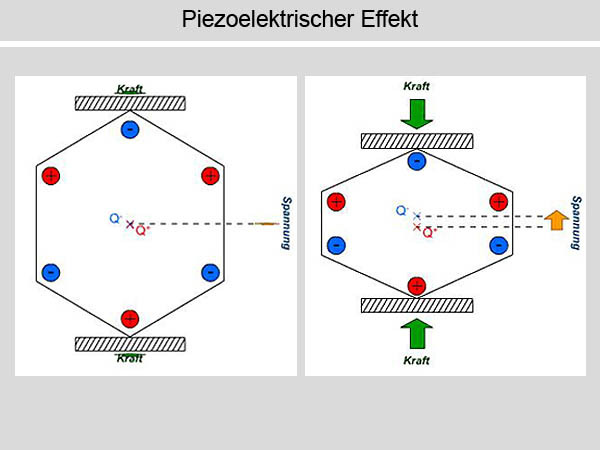
\includegraphics[width=0.6\textwidth]{Abb/piezo.jpg}
    \caption{Piezoelektrischer Effekt [https://vetsuisse.com/vet-iml/lernmodule/htmls/slide.html?radiosurfvet|radgeneral|sonography|sonobasics|2]}
    \label{piezo}
\end{figure}

Kehrt man dieses Prinzip nun um (inverser piezoelektrischer Effekt), also legt man Spannung an solch einer Kristallstruktur an, lassen sich nun mechanische Verfromungen, mit diesen Kristallen, über elektrische Kräfte erzeugen.
Man nutzt diesen Effekt bei der Rastereinheit, da sich so sehr exakte und minimale Änderungen in x-, y- und z-Richtung erzeugen lassen.
Typische Rasterbereiche sind $10-\SI{100}{\mu m}$ in x- und y-Richtung und $2-\SI{5}{\mu m}$ in z-Richtung.
Das hier verwendete Mikroskop basiert auf diesem elektromechanischem Prinzip, also der Deformierung der piezoelektrischen Materialien zur feineren Bewegung des Cantilevers.
Alternativ lässt sich auch die Probe bewegen.




 \subsection{Detektionseinheit}
 
 Das in diesem Versuch verwendete EasyScan DFM Rasterkraftmiskroskop nutzt zur Auslesung der Amplitudenänderung ein optisches Verfahren. 
 Man verwendet einen Laser, der auf die Rückseite des Cantilevers ausgerichtet ist, wo sich eine polierte Stelle befindet, welche das Licht des Lasers spiegelt.
 Bei der Deformation des Cantilevers ändert sich somit die Position des gespiegelten Lichtbündels.
 Mithilfe einer Photodiode lassen sich diese minimalen Änderungen sehr gut messen und in Größenordnungen von einzelnen Angstrøm umrechnen.
 Diese Methode eignet sich hervorragend, denn das Laserlicht wird lediglich durch Erschütterungen gestört.
 Deshalb baut man diesen Versuch auf einem massiven Steintisch auf und versucht Erschütterungen bei der Messung zu vermeiden.

